% Options for packages loaded elsewhere
\PassOptionsToPackage{unicode}{hyperref}
\PassOptionsToPackage{hyphens}{url}
%
\documentclass[
]{article}
\usepackage{lmodern}
\usepackage{amssymb,amsmath}
\usepackage{ifxetex,ifluatex}
\ifnum 0\ifxetex 1\fi\ifluatex 1\fi=0 % if pdftex
  \usepackage[T1]{fontenc}
  \usepackage[utf8]{inputenc}
  \usepackage{textcomp} % provide euro and other symbols
\else % if luatex or xetex
  \usepackage{unicode-math}
  \defaultfontfeatures{Scale=MatchLowercase}
  \defaultfontfeatures[\rmfamily]{Ligatures=TeX,Scale=1}
\fi
% Use upquote if available, for straight quotes in verbatim environments
\IfFileExists{upquote.sty}{\usepackage{upquote}}{}
\IfFileExists{microtype.sty}{% use microtype if available
  \usepackage[]{microtype}
  \UseMicrotypeSet[protrusion]{basicmath} % disable protrusion for tt fonts
}{}
\makeatletter
\@ifundefined{KOMAClassName}{% if non-KOMA class
  \IfFileExists{parskip.sty}{%
    \usepackage{parskip}
  }{% else
    \setlength{\parindent}{0pt}
    \setlength{\parskip}{6pt plus 2pt minus 1pt}}
}{% if KOMA class
  \KOMAoptions{parskip=half}}
\makeatother
\usepackage{xcolor}
\IfFileExists{xurl.sty}{\usepackage{xurl}}{} % add URL line breaks if available
\IfFileExists{bookmark.sty}{\usepackage{bookmark}}{\usepackage{hyperref}}
\hypersetup{
  pdftitle={Homework 1 Solutions},
  pdfauthor={Gurdeep Singh},
  hidelinks,
  pdfcreator={LaTeX via pandoc}}
\urlstyle{same} % disable monospaced font for URLs
\usepackage[margin=1in]{geometry}
\usepackage{color}
\usepackage{fancyvrb}
\newcommand{\VerbBar}{|}
\newcommand{\VERB}{\Verb[commandchars=\\\{\}]}
\DefineVerbatimEnvironment{Highlighting}{Verbatim}{commandchars=\\\{\}}
% Add ',fontsize=\small' for more characters per line
\usepackage{framed}
\definecolor{shadecolor}{RGB}{248,248,248}
\newenvironment{Shaded}{\begin{snugshade}}{\end{snugshade}}
\newcommand{\AlertTok}[1]{\textcolor[rgb]{0.94,0.16,0.16}{#1}}
\newcommand{\AnnotationTok}[1]{\textcolor[rgb]{0.56,0.35,0.01}{\textbf{\textit{#1}}}}
\newcommand{\AttributeTok}[1]{\textcolor[rgb]{0.77,0.63,0.00}{#1}}
\newcommand{\BaseNTok}[1]{\textcolor[rgb]{0.00,0.00,0.81}{#1}}
\newcommand{\BuiltInTok}[1]{#1}
\newcommand{\CharTok}[1]{\textcolor[rgb]{0.31,0.60,0.02}{#1}}
\newcommand{\CommentTok}[1]{\textcolor[rgb]{0.56,0.35,0.01}{\textit{#1}}}
\newcommand{\CommentVarTok}[1]{\textcolor[rgb]{0.56,0.35,0.01}{\textbf{\textit{#1}}}}
\newcommand{\ConstantTok}[1]{\textcolor[rgb]{0.00,0.00,0.00}{#1}}
\newcommand{\ControlFlowTok}[1]{\textcolor[rgb]{0.13,0.29,0.53}{\textbf{#1}}}
\newcommand{\DataTypeTok}[1]{\textcolor[rgb]{0.13,0.29,0.53}{#1}}
\newcommand{\DecValTok}[1]{\textcolor[rgb]{0.00,0.00,0.81}{#1}}
\newcommand{\DocumentationTok}[1]{\textcolor[rgb]{0.56,0.35,0.01}{\textbf{\textit{#1}}}}
\newcommand{\ErrorTok}[1]{\textcolor[rgb]{0.64,0.00,0.00}{\textbf{#1}}}
\newcommand{\ExtensionTok}[1]{#1}
\newcommand{\FloatTok}[1]{\textcolor[rgb]{0.00,0.00,0.81}{#1}}
\newcommand{\FunctionTok}[1]{\textcolor[rgb]{0.00,0.00,0.00}{#1}}
\newcommand{\ImportTok}[1]{#1}
\newcommand{\InformationTok}[1]{\textcolor[rgb]{0.56,0.35,0.01}{\textbf{\textit{#1}}}}
\newcommand{\KeywordTok}[1]{\textcolor[rgb]{0.13,0.29,0.53}{\textbf{#1}}}
\newcommand{\NormalTok}[1]{#1}
\newcommand{\OperatorTok}[1]{\textcolor[rgb]{0.81,0.36,0.00}{\textbf{#1}}}
\newcommand{\OtherTok}[1]{\textcolor[rgb]{0.56,0.35,0.01}{#1}}
\newcommand{\PreprocessorTok}[1]{\textcolor[rgb]{0.56,0.35,0.01}{\textit{#1}}}
\newcommand{\RegionMarkerTok}[1]{#1}
\newcommand{\SpecialCharTok}[1]{\textcolor[rgb]{0.00,0.00,0.00}{#1}}
\newcommand{\SpecialStringTok}[1]{\textcolor[rgb]{0.31,0.60,0.02}{#1}}
\newcommand{\StringTok}[1]{\textcolor[rgb]{0.31,0.60,0.02}{#1}}
\newcommand{\VariableTok}[1]{\textcolor[rgb]{0.00,0.00,0.00}{#1}}
\newcommand{\VerbatimStringTok}[1]{\textcolor[rgb]{0.31,0.60,0.02}{#1}}
\newcommand{\WarningTok}[1]{\textcolor[rgb]{0.56,0.35,0.01}{\textbf{\textit{#1}}}}
\usepackage{graphicx,grffile}
\makeatletter
\def\maxwidth{\ifdim\Gin@nat@width>\linewidth\linewidth\else\Gin@nat@width\fi}
\def\maxheight{\ifdim\Gin@nat@height>\textheight\textheight\else\Gin@nat@height\fi}
\makeatother
% Scale images if necessary, so that they will not overflow the page
% margins by default, and it is still possible to overwrite the defaults
% using explicit options in \includegraphics[width, height, ...]{}
\setkeys{Gin}{width=\maxwidth,height=\maxheight,keepaspectratio}
% Set default figure placement to htbp
\makeatletter
\def\fps@figure{htbp}
\makeatother
\setlength{\emergencystretch}{3em} % prevent overfull lines
\providecommand{\tightlist}{%
  \setlength{\itemsep}{0pt}\setlength{\parskip}{0pt}}
\setcounter{secnumdepth}{-\maxdimen} % remove section numbering

\title{Homework 1 Solutions}
\author{Gurdeep Singh}
\date{9/14/2020}

\begin{document}
\maketitle

\hypertarget{problem-1}{%
\subsection{Problem 1}\label{problem-1}}

\begin{verbatim}
Refer to the Grade point average Data. The director of admissions of a small college selected 120 students at random from the new freshman class in a study to determine whether a student's grade point average (GPA) at the end of the freshman year (Y) can be predicted from the ACT test score (X). (30 points)
\end{verbatim}

a-)Obtain the least squares estimates of \(\beta_{0}\) and
\(\beta_{1}\), and state the estimated regression function. (5pts)\\
b-) Plot the estimated regression function and the data. "Does the
estimated regression function appear to fit the data well? (5pts)\\
c-)Obtain a point estimate of the mean freshman GPA for students with
ACT test score X = 30. (5pts)\\
d-)What is the point estimate of the change in the mean response when
the entrance test score increases by one point? (5pts)\\
e-)Obtain the residuals \(\epsilon_{i}\). Do they sum to zero? (5pts)\\
f-)Estimate \(\sigma\)\^{}2 and \(\sigma\). In what units is σ
expressed? (5pts)\\

\hypertarget{solutions}{%
\section{Solutions:}\label{solutions}}

a-) Solution:

\begin{Shaded}
\begin{Highlighting}[]
\KeywordTok{library}\NormalTok{(knitr)}

\CommentTok{# read in data}
\NormalTok{gpa <-}\StringTok{ }\KeywordTok{read.csv}\NormalTok{(}\StringTok{"/cloud/project/HW1/Grade Point Average Data.csv"}\NormalTok{)}
\KeywordTok{colnames}\NormalTok{(gpa) =}\StringTok{ }\KeywordTok{c}\NormalTok{(}\StringTok{'student_gpa'}\NormalTok{, }\StringTok{'act_score'}\NormalTok{)}
\KeywordTok{head}\NormalTok{(gpa)}
\end{Highlighting}
\end{Shaded}

\begin{verbatim}
##   student_gpa act_score
## 1       3.897        21
## 2       3.885        14
## 3       3.778        28
## 4       2.540        22
## 5       3.028        21
## 6       3.865        31
\end{verbatim}

\begin{Shaded}
\begin{Highlighting}[]
\CommentTok{# fit regression, obtain coefficients and residuals}
\NormalTok{reg_q1 <-}\StringTok{ }\KeywordTok{lm}\NormalTok{(student_gpa}\OperatorTok{~}\NormalTok{act_score, }\DataTypeTok{data =}\NormalTok{ gpa)}
\KeywordTok{print}\NormalTok{(reg_q1}\OperatorTok{$}\NormalTok{coefficients)}
\end{Highlighting}
\end{Shaded}

\begin{verbatim}
## (Intercept)   act_score 
##  2.11404929  0.03882713
\end{verbatim}

\begin{Shaded}
\begin{Highlighting}[]
\NormalTok{intercept_q1 =}\StringTok{ }\NormalTok{reg_q1}\OperatorTok{$}\NormalTok{coefficients[}\DecValTok{1}\NormalTok{]}
\NormalTok{act_score_q1 =}\StringTok{ }\NormalTok{reg_q1}\OperatorTok{$}\NormalTok{coefficients[}\DecValTok{2}\NormalTok{]}
\NormalTok{res_q1 =}\StringTok{ }\NormalTok{reg_q1}\OperatorTok{$}\NormalTok{residuals}
\end{Highlighting}
\end{Shaded}

As seen above, the coefficients are \(\beta_0\) = 2.11404929 and
\(\beta_1\) = 0.03882713

\begin{enumerate}
\def\labelenumi{\alph{enumi})}
\setcounter{enumi}{1}
\tightlist
\item
  Solution:
\end{enumerate}

\begin{Shaded}
\begin{Highlighting}[]
\KeywordTok{library}\NormalTok{(knitr)}

\KeywordTok{plot}\NormalTok{(gpa}\OperatorTok{$}\NormalTok{act_score, gpa}\OperatorTok{$}\NormalTok{student_gpa, }\DataTypeTok{xlab =} \StringTok{"ACT Test Score"}\NormalTok{, }\DataTypeTok{ylab =} \StringTok{"GPA"}\NormalTok{)}
\KeywordTok{abline}\NormalTok{(reg_q1, }\DataTypeTok{col =} \StringTok{'red'}\NormalTok{)}
\end{Highlighting}
\end{Shaded}

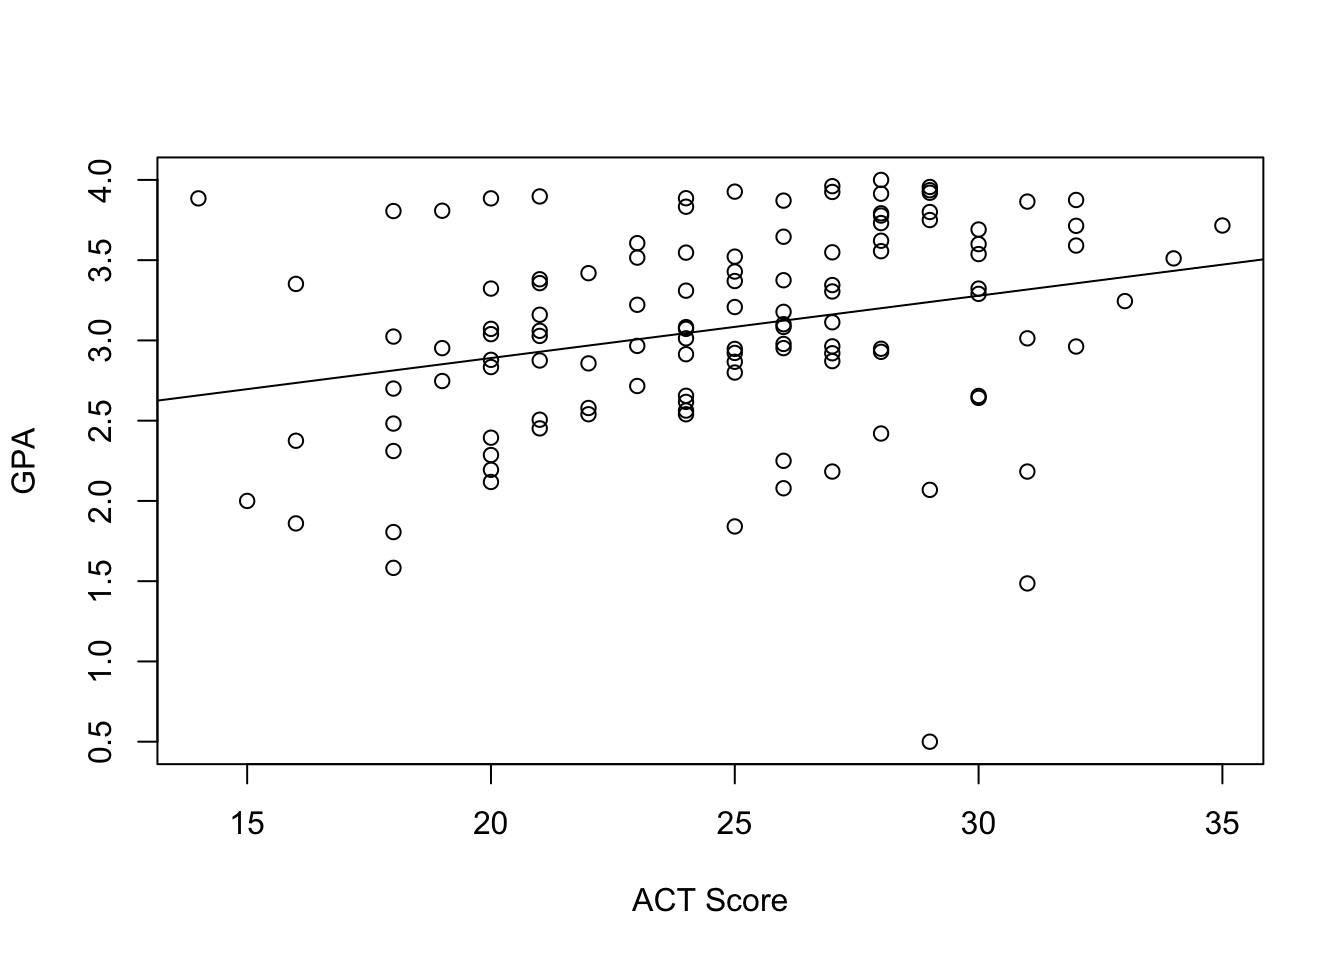
\includegraphics{CSCI-E-106-Fall-2020-Homework-1-Template_files/figure-latex/unnamed-chunk-2-1.pdf}

As seen above the points are widely distributed and not clustered around
the line. Hence the estimated regression function is not a good fit for
the data provided.

\begin{enumerate}
\def\labelenumi{\alph{enumi})}
\setcounter{enumi}{2}
\tightlist
\item
  Solution:
\end{enumerate}

\begin{Shaded}
\begin{Highlighting}[]
\NormalTok{act_score =}\StringTok{ }\DecValTok{30}
\NormalTok{mean_freshman_gpa =}\StringTok{ }\NormalTok{intercept_q1 }\OperatorTok{+}\StringTok{ }\NormalTok{(act_score }\OperatorTok{*}\StringTok{ }\NormalTok{act_score_q1)}
\NormalTok{mean_freshman_gpa}
\end{Highlighting}
\end{Shaded}

\begin{verbatim}
## (Intercept) 
##    3.278863
\end{verbatim}

Point estimate of the mean freshman GPA for students with score 30 is
3.278863

\begin{enumerate}
\def\labelenumi{\alph{enumi})}
\setcounter{enumi}{3}
\tightlist
\item
  Solution:
\end{enumerate}

\begin{Shaded}
\begin{Highlighting}[]
\KeywordTok{print}\NormalTok{(act_score_q1)}
\end{Highlighting}
\end{Shaded}

\begin{verbatim}
##  act_score 
## 0.03882713
\end{verbatim}

For a 1 point increase in entrance test score the GPA increases by the
\(beta_1\) coefficient = 0.0388 points

\begin{enumerate}
\def\labelenumi{\alph{enumi})}
\setcounter{enumi}{4}
\tightlist
\item
  Solution:
\end{enumerate}

\begin{Shaded}
\begin{Highlighting}[]
\NormalTok{res_q1[}\DecValTok{1}\OperatorTok{:}\DecValTok{10}\NormalTok{] }\CommentTok{# residuals were calculated in 1a; printing 1st 10 variables here}
\end{Highlighting}
\end{Shaded}

\begin{verbatim}
##           1           2           3           4           5           6 
##  0.96758105  1.22737094  0.57679116 -0.42824608  0.09858105  0.54730978 
##           7           8           9          10 
## -0.39451735  0.79861829 -2.74003597  0.05444541
\end{verbatim}

\begin{Shaded}
\begin{Highlighting}[]
\NormalTok{ssr_q1 =}\StringTok{ }\KeywordTok{sum}\NormalTok{(res_q1)}
\KeywordTok{print}\NormalTok{(ssr_q1)}
\end{Highlighting}
\end{Shaded}

\begin{verbatim}
## [1] -7.2789e-15
\end{verbatim}

The residuals are not exactly zero but a very small value as seen above
and can be considered as summing to zero for all practical purposes.

\begin{enumerate}
\def\labelenumi{\alph{enumi})}
\setcounter{enumi}{5}
\tightlist
\item
  Solution:
\end{enumerate}

\begin{Shaded}
\begin{Highlighting}[]
\NormalTok{ei2 =}\StringTok{ }\KeywordTok{sum}\NormalTok{((res_q1)}\OperatorTok{^}\DecValTok{2}\NormalTok{)}
\NormalTok{sigma2 =}\StringTok{ }\NormalTok{ei2}\OperatorTok{/}\NormalTok{(}\KeywordTok{length}\NormalTok{(res_q1)}\OperatorTok{-}\DecValTok{2}\NormalTok{)}
\NormalTok{sigma =}\StringTok{ }\KeywordTok{sqrt}\NormalTok{(sigma2)}

\KeywordTok{print}\NormalTok{(sigma2)}
\end{Highlighting}
\end{Shaded}

\begin{verbatim}
## [1] 0.3882848
\end{verbatim}

\begin{Shaded}
\begin{Highlighting}[]
\KeywordTok{print}\NormalTok{(sigma)}
\end{Highlighting}
\end{Shaded}

\begin{verbatim}
## [1] 0.623125
\end{verbatim}

\(\sigma\) is expressed in units of GPA

\hypertarget{problem-2}{%
\subsection{Problem 2}\label{problem-2}}

Typographical errors shown below are the number of galleys for a
manuscript (X) and the dollar cost of correcting typographical errors
(Y) in a random sample of recent orders handled by a firm specializing
in technical manuscripts. Assume that the regression model Yi = β1X1 +
ε\_i is appropriate, with normally distributed independent error terms
whose variance is a σ\^{}2 = 16. (20 pts)

\begin{enumerate}
\def\labelenumi{\alph{enumi})}
\item
  Evaluate the likelihood function for \(\beta_{1}= 1,2, 3,…,100\). For
  which of \(\beta_{1}\) values is the likelihood function largest?
  (10pts)\\
\item
  The maximum likelihood estimator is
  \(b_{1}=\sum X_{i} Y_{i}/\sum X_{i}^2\). Find the maximum likelihood
  estimate. Are your results in part (a) consistent with this estimate?
  (10 pts)\\
\end{enumerate}

\hypertarget{solutions-1}{%
\subsection{Solutions:}\label{solutions-1}}

\begin{enumerate}
\def\labelenumi{\alph{enumi})}
\item
\end{enumerate}

\begin{Shaded}
\begin{Highlighting}[]
\CommentTok{# input data}
\NormalTok{x_num_galley <-}\StringTok{ }\KeywordTok{c}\NormalTok{(}\DecValTok{7}\NormalTok{, }\DecValTok{12}\NormalTok{, }\DecValTok{4}\NormalTok{, }\DecValTok{14}\NormalTok{, }\DecValTok{25}\NormalTok{, }\DecValTok{30}\NormalTok{)}
\NormalTok{y_corr_cost <-}\StringTok{ }\KeywordTok{c}\NormalTok{(}\DecValTok{128}\NormalTok{, }\DecValTok{213}\NormalTok{, }\DecValTok{75}\NormalTok{, }\DecValTok{250}\NormalTok{, }\DecValTok{446}\NormalTok{, }\DecValTok{540}\NormalTok{)}
\NormalTok{n_beta <-}\StringTok{ }\DecValTok{100}
\NormalTok{sig2_err <-}\StringTok{ }\DecValTok{16} \CommentTok{# variance given}


\CommentTok{# empty vectors to store output; len = n_beta to store all likelihood values}
\NormalTok{lkhood_val <-}\StringTok{ }\KeywordTok{vector}\NormalTok{(}\DataTypeTok{mode =} \StringTok{'integer'}\NormalTok{, }\DataTypeTok{length =}\NormalTok{ n_beta) }

\ControlFlowTok{for}\NormalTok{ (beta_val }\ControlFlowTok{in} \DecValTok{1}\OperatorTok{:}\StringTok{ }\NormalTok{n_beta) \{}
  \CommentTok{#print(beta_val)}
\NormalTok{  interim1 <-}\StringTok{  }\NormalTok{beta_val }\OperatorTok{*}\StringTok{ }\NormalTok{x_num_galley}
\NormalTok{  interim2 <-}\StringTok{  }\NormalTok{(y_corr_cost }\OperatorTok{-}\StringTok{ }\NormalTok{interim1)}\OperatorTok{^}\DecValTok{2}
\NormalTok{  interim3 <-}\StringTok{  }\KeywordTok{sum}\NormalTok{(interim2)}
\NormalTok{  interim4 <-}\StringTok{ }\KeywordTok{exp}\NormalTok{(interim3}\OperatorTok{/}\NormalTok{(}\OperatorTok{-}\DecValTok{2}\OperatorTok{*}\NormalTok{sig2_err))}
\NormalTok{  interim5 <-}\StringTok{ }\NormalTok{interim4}\OperatorTok{/}\NormalTok{((}\DecValTok{2}\OperatorTok{*}\NormalTok{pi}\OperatorTok{*}\NormalTok{sig2_err)}\OperatorTok{^}\NormalTok{(}\KeywordTok{length}\NormalTok{(x_num_galley)}\OperatorTok{/}\DecValTok{2}\NormalTok{))}
\NormalTok{  lkhood_val[beta_val] <-}\StringTok{ }\NormalTok{interim5}
\NormalTok{\}}

\CommentTok{# get index of value which has maximum value of likelihood}
\CommentTok{# max index value corresponds to beta}
\KeywordTok{which.max}\NormalTok{(lkhood_val)}
\end{Highlighting}
\end{Shaded}

\begin{verbatim}
## [1] 18
\end{verbatim}

Value of likelihood function is largest for \(\beta_1\) = 18

\begin{enumerate}
\def\labelenumi{\alph{enumi})}
\setcounter{enumi}{1}
\item
\end{enumerate}

\begin{Shaded}
\begin{Highlighting}[]
\NormalTok{mle_2b <-}\StringTok{ }\KeywordTok{sum}\NormalTok{(x_num_galley}\OperatorTok{*}\NormalTok{y_corr_cost)}\OperatorTok{/}\KeywordTok{sum}\NormalTok{(x_num_galley }\OperatorTok{*}\StringTok{ }\NormalTok{x_num_galley)}
\NormalTok{mle_2b}
\end{Highlighting}
\end{Shaded}

\begin{verbatim}
## [1] 17.9285
\end{verbatim}

As seen above the results in part 2a and part 2b are consistent.

\hypertarget{problem-3}{%
\subsection{Problem 3}\label{problem-3}}

Refer to the CDI data set. The number of active physicians in a CDI (Y)
is expected to be related to total population, number of hospital beds,
and total personal income. (30 points)

\begin{enumerate}
\def\labelenumi{\alph{enumi})}
\tightlist
\item
  Regress the number of active physicians in turn on each of the three
  predictor variables. State the estimated regression functions. (10
  points)\\
\item
  Plot the three estimated regression functions and data on separate
  graphs. Does a linear regression relation appear to provide a good fit
  for each of the three predictor variables? (10 points)\\
\item
  Calculate MSE for each of the three predictor variables. Which
  predictor variable leads to the smallest variability around the fitted
  regression line? Which variable would you use the estimate Y and why?
  (10 points)\\
\end{enumerate}

\hypertarget{solutions-2}{%
\subsection{Solutions}\label{solutions-2}}

\begin{enumerate}
\def\labelenumi{\alph{enumi})}
\item
\end{enumerate}

\begin{Shaded}
\begin{Highlighting}[]
\CommentTok{# read in data}
\NormalTok{cdi <-}\StringTok{ }\KeywordTok{read.csv}\NormalTok{(}\StringTok{"/cloud/project/HW1/CDI Data.csv"}\NormalTok{)}
\KeywordTok{head}\NormalTok{(cdi)}
\end{Highlighting}
\end{Shaded}

\begin{verbatim}
##   Identification.number      County State Land.area Total.population
## 1                     1 Los_Angeles    CA      4060          8863164
## 2                     2        Cook    IL       946          5105067
## 3                     3      Harris    TX      1729          2818199
## 4                     4   San_Diego    CA      4205          2498016
## 5                     5      Orange    CA       790          2410556
## 6                     6       Kings    NY        71          2300664
##   Percent.of.population.aged.18.34 Percent.of.population.65.or.older
## 1                             32.1                               9.7
## 2                             29.2                              12.4
## 3                             31.3                               7.1
## 4                             33.5                              10.9
## 5                             32.6                               9.2
## 6                             28.3                              12.4
##   Number.of.active.physicians Number.of.hospital.beds Total.serious.crimes
## 1                       23677                   27700               688936
## 2                       15153                   21550               436936
## 3                        7553                   12449               253526
## 4                        5905                    6179               173821
## 5                        6062                    6369               144524
## 6                        4861                    8942               680966
##   Percent.high.school.graduates Percent.bachelor.s.degrees
## 1                          70.0                       22.3
## 2                          73.4                       22.8
## 3                          74.9                       25.4
## 4                          81.9                       25.3
## 5                          81.2                       27.8
## 6                          63.7                       16.6
##   Percent.below.poverty.level Percent.unemployment Per.capita.income
## 1                        11.6                  8.0             20786
## 2                        11.1                  7.2             21729
## 3                        12.5                  5.7             19517
## 4                         8.1                  6.1             19588
## 5                         5.2                  4.8             24400
## 6                        19.5                  9.5             16803
##   Total.personal.income Geographic.region
## 1                184230                 4
## 2                110928                 2
## 3                 55003                 3
## 4                 48931                 4
## 5                 58818                 4
## 6                 38658                 1
\end{verbatim}

\begin{Shaded}
\begin{Highlighting}[]
\KeywordTok{colnames}\NormalTok{(cdi)}
\end{Highlighting}
\end{Shaded}

\begin{verbatim}
##  [1] "Identification.number"             "County"                           
##  [3] "State"                             "Land.area"                        
##  [5] "Total.population"                  "Percent.of.population.aged.18.34" 
##  [7] "Percent.of.population.65.or.older" "Number.of.active.physicians"      
##  [9] "Number.of.hospital.beds"           "Total.serious.crimes"             
## [11] "Percent.high.school.graduates"     "Percent.bachelor.s.degrees"       
## [13] "Percent.below.poverty.level"       "Percent.unemployment"             
## [15] "Per.capita.income"                 "Total.personal.income"            
## [17] "Geographic.region"
\end{verbatim}

\begin{Shaded}
\begin{Highlighting}[]
\CommentTok{# fit regression separately for each variable specified in the question}
\NormalTok{reg_q2_tot_pop <-}\StringTok{ }\KeywordTok{lm}\NormalTok{(Number.of.active.physicians}\OperatorTok{~}\NormalTok{Total.population, }\DataTypeTok{data =}\NormalTok{ cdi)}
\NormalTok{reg_q2_tot_pop}\OperatorTok{$}\NormalTok{coefficients}
\end{Highlighting}
\end{Shaded}

\begin{verbatim}
##      (Intercept) Total.population 
##    -1.106348e+02     2.795425e-03
\end{verbatim}

\begin{Shaded}
\begin{Highlighting}[]
\NormalTok{reg_q2_num_beds <-}\StringTok{ }\KeywordTok{lm}\NormalTok{(Number.of.active.physicians}\OperatorTok{~}\NormalTok{Number.of.hospital.beds, }\DataTypeTok{data =}\NormalTok{ cdi)}
\NormalTok{reg_q2_num_beds}\OperatorTok{$}\NormalTok{coefficients}
\end{Highlighting}
\end{Shaded}

\begin{verbatim}
##             (Intercept) Number.of.hospital.beds 
##             -95.9321847               0.7431164
\end{verbatim}

\begin{Shaded}
\begin{Highlighting}[]
\NormalTok{reg_q2_tot_income <-}\StringTok{ }\KeywordTok{lm}\NormalTok{(Number.of.active.physicians}\OperatorTok{~}\NormalTok{Total.personal.income, }\DataTypeTok{data =}\NormalTok{ cdi)}
\NormalTok{reg_q2_tot_income}\OperatorTok{$}\NormalTok{coefficients}
\end{Highlighting}
\end{Shaded}

\begin{verbatim}
##           (Intercept) Total.personal.income 
##           -48.3948489             0.1317012
\end{verbatim}

The estimated regression functions are as below:

Number.of.active.physicians = -1.106348e+02 + 2.795425e-03 *
Total.population

Number.of.active.physicians = -95.9321847 + 0.7431164 *
Number.of.hospital.beds

Number.of.active.physicians = -48.3948489 + 0.1317012 *
Total.personal.income b)

\begin{Shaded}
\begin{Highlighting}[]
\KeywordTok{plot}\NormalTok{(cdi}\OperatorTok{$}\NormalTok{Total.population, cdi}\OperatorTok{$}\NormalTok{Number.of.active.physicians, }\DataTypeTok{xlab =} \StringTok{'Total Population'}\NormalTok{, }\DataTypeTok{ylab =} \StringTok{'Number of Active Physicians'}\NormalTok{)}
\KeywordTok{abline}\NormalTok{(reg_q2_tot_pop, }\DataTypeTok{col =} \StringTok{'red'}\NormalTok{)}
\end{Highlighting}
\end{Shaded}

\includegraphics{CSCI-E-106-Fall-2020-Homework-1-Template_files/figure-latex/unnamed-chunk-10-1.pdf}

\begin{Shaded}
\begin{Highlighting}[]
\KeywordTok{plot}\NormalTok{(cdi}\OperatorTok{$}\NormalTok{Number.of.hospital.beds, cdi}\OperatorTok{$}\NormalTok{Number.of.active.physicians, }\DataTypeTok{xlab =} \StringTok{'Number of Hospital beds'}\NormalTok{, }\DataTypeTok{ylab =} \StringTok{'Number of Active Physicians'}\NormalTok{)}
\KeywordTok{abline}\NormalTok{(reg_q2_num_beds, }\DataTypeTok{col =} \StringTok{'red'}\NormalTok{)}
\end{Highlighting}
\end{Shaded}

\includegraphics{CSCI-E-106-Fall-2020-Homework-1-Template_files/figure-latex/unnamed-chunk-10-2.pdf}

\begin{Shaded}
\begin{Highlighting}[]
\KeywordTok{plot}\NormalTok{(cdi}\OperatorTok{$}\NormalTok{Total.personal.income, cdi}\OperatorTok{$}\NormalTok{Number.of.active.physicians, }\DataTypeTok{xlab =} \StringTok{'Total Personal Income'}\NormalTok{, }\DataTypeTok{ylab =} \StringTok{'Number of Active Physicians'}\NormalTok{)}
\KeywordTok{abline}\NormalTok{(reg_q2_tot_income, }\DataTypeTok{col =} \StringTok{'red'}\NormalTok{)}
\end{Highlighting}
\end{Shaded}

\includegraphics{CSCI-E-106-Fall-2020-Homework-1-Template_files/figure-latex/unnamed-chunk-10-3.pdf}
From a visual inspection of the graphs the regression lines do appear to
be a good fit for each of the predictor variables; though in all cases
the data points are clustered towards the start of the x-axis.

Hence, some form of outlier removal and/or log transformation might be
appropriate here.

\begin{enumerate}
\def\labelenumi{\alph{enumi})}
\setcounter{enumi}{2}
\item
\end{enumerate}

\begin{Shaded}
\begin{Highlighting}[]
\NormalTok{sse_q2_num_beds =}\StringTok{ }\KeywordTok{sum}\NormalTok{((reg_q2_num_beds}\OperatorTok{$}\NormalTok{residuals)}\OperatorTok{^}\DecValTok{2}\NormalTok{)}
\NormalTok{mse_q2_num_beds =}\StringTok{ }\NormalTok{sse_q2_num_beds}\OperatorTok{/}\NormalTok{(}\KeywordTok{length}\NormalTok{(reg_q2_num_beds}\OperatorTok{$}\NormalTok{residuals)}\OperatorTok{-}\DecValTok{2}\NormalTok{)}
\NormalTok{mse_q2_num_beds}
\end{Highlighting}
\end{Shaded}

\begin{verbatim}
## [1] 310191.9
\end{verbatim}

\begin{Shaded}
\begin{Highlighting}[]
\NormalTok{sse_q2_tot_income =}\StringTok{ }\KeywordTok{sum}\NormalTok{((reg_q2_tot_income}\OperatorTok{$}\NormalTok{residuals)}\OperatorTok{^}\DecValTok{2}\NormalTok{)}
\NormalTok{mse_q2_tot_income =}\StringTok{ }\NormalTok{sse_q2_tot_income}\OperatorTok{/}\NormalTok{(}\KeywordTok{length}\NormalTok{(reg_q2_tot_income}\OperatorTok{$}\NormalTok{residuals)}\OperatorTok{-}\DecValTok{2}\NormalTok{)}
\NormalTok{mse_q2_tot_income}
\end{Highlighting}
\end{Shaded}

\begin{verbatim}
## [1] 324539.4
\end{verbatim}

\begin{Shaded}
\begin{Highlighting}[]
\NormalTok{sse_q2_tot_pop =}\StringTok{ }\KeywordTok{sum}\NormalTok{((reg_q2_tot_pop}\OperatorTok{$}\NormalTok{residuals)}\OperatorTok{^}\DecValTok{2}\NormalTok{)}
\NormalTok{mse_q2_tot_pop =}\StringTok{ }\NormalTok{sse_q2_tot_pop}\OperatorTok{/}\NormalTok{(}\KeywordTok{length}\NormalTok{(reg_q2_tot_pop}\OperatorTok{$}\NormalTok{residuals)}\OperatorTok{-}\DecValTok{2}\NormalTok{)}
\NormalTok{mse_q2_tot_pop}
\end{Highlighting}
\end{Shaded}

\begin{verbatim}
## [1] 372203.5
\end{verbatim}

Number of beds has the lowest mean square error. I would use this
variable since of the 3 given to us this has the lowest overall
deviation from given values.

\hypertarget{problem-4}{%
\subsection{Problem 4}\label{problem-4}}

Refer to the CDI data set. Use the number of active physicians as Y and
total personal income as X. Select 1,000 random samples of 400
observations, fit the regression model and record \(\beta_{0}\) and
\(\beta_{1}\) for each selected sample. Calculate the mean and variance
of \(\beta_{0}\) and \(\beta_{1}\) based on the 1,000 different
regression line and compare against the regression model in question 3
part a. (20 points)

\hypertarget{solution}{%
\subsection{Solution:}\label{solution}}

\begin{Shaded}
\begin{Highlighting}[]
\CommentTok{# create new DF with columns of interest}
\KeywordTok{colnames}\NormalTok{(cdi) }\CommentTok{# to get index numbers of columns to copy into new DF}
\end{Highlighting}
\end{Shaded}

\begin{verbatim}
##  [1] "Identification.number"             "County"                           
##  [3] "State"                             "Land.area"                        
##  [5] "Total.population"                  "Percent.of.population.aged.18.34" 
##  [7] "Percent.of.population.65.or.older" "Number.of.active.physicians"      
##  [9] "Number.of.hospital.beds"           "Total.serious.crimes"             
## [11] "Percent.high.school.graduates"     "Percent.bachelor.s.degrees"       
## [13] "Percent.below.poverty.level"       "Percent.unemployment"             
## [15] "Per.capita.income"                 "Total.personal.income"            
## [17] "Geographic.region"
\end{verbatim}

\begin{Shaded}
\begin{Highlighting}[]
\NormalTok{df_q4 <-}\StringTok{ }\NormalTok{cdi[,}\KeywordTok{c}\NormalTok{(}\DecValTok{8}\NormalTok{, }\DecValTok{16}\NormalTok{)]}
\KeywordTok{head}\NormalTok{(df_q4)}
\end{Highlighting}
\end{Shaded}

\begin{verbatim}
##   Number.of.active.physicians Total.personal.income
## 1                       23677                184230
## 2                       15153                110928
## 3                        7553                 55003
## 4                        5905                 48931
## 5                        6062                 58818
## 6                        4861                 38658
\end{verbatim}

\begin{Shaded}
\begin{Highlighting}[]
\CommentTok{# specify parameters and blank vectors to store output}
\KeywordTok{set.seed}\NormalTok{(}\DecValTok{123}\NormalTok{)}
\NormalTok{n_obs <-}\StringTok{ }\DecValTok{400}
\NormalTok{n_samples <-}\StringTok{ }\DecValTok{1000}
\NormalTok{beta0_q4 <-}\StringTok{ }\KeywordTok{vector}\NormalTok{(}\DataTypeTok{mode =} \StringTok{'integer'}\NormalTok{, }\DataTypeTok{length =}\NormalTok{ n_samples)}
\NormalTok{beta1_q4 <-}\StringTok{ }\KeywordTok{vector}\NormalTok{(}\DataTypeTok{mode =} \StringTok{'integer'}\NormalTok{, }\DataTypeTok{length =}\NormalTok{ n_samples)}

\ControlFlowTok{for}\NormalTok{ (i }\ControlFlowTok{in} \DecValTok{1}\OperatorTok{:}\NormalTok{n_samples) \{}
  \CommentTok{# print(i)}
\NormalTok{  q4_index <-}\StringTok{ }\KeywordTok{sample}\NormalTok{(}\DecValTok{1}\OperatorTok{:}\KeywordTok{nrow}\NormalTok{(df_q4), n_obs)}
\NormalTok{  q4_sample_df <-}\StringTok{ }\NormalTok{df_q4[q4_index,]}
\NormalTok{  q4_sample_reg <-}\StringTok{ }\KeywordTok{lm}\NormalTok{(Number.of.active.physicians}\OperatorTok{~}\NormalTok{Total.personal.income, }\DataTypeTok{data =}\NormalTok{ q4_sample_df)}
\NormalTok{  beta0_q4[i] <-}\StringTok{ }\NormalTok{q4_sample_reg}\OperatorTok{$}\NormalTok{coefficients[}\DecValTok{1}\NormalTok{]}
\NormalTok{  beta1_q4[i] <-}\StringTok{ }\NormalTok{q4_sample_reg}\OperatorTok{$}\NormalTok{coefficients[}\DecValTok{2}\NormalTok{]}
\NormalTok{\}}

\NormalTok{q4_beta0_mean <-}\StringTok{ }\KeywordTok{mean}\NormalTok{(beta0_q4)}
\KeywordTok{print}\NormalTok{(q4_beta0_mean)}
\end{Highlighting}
\end{Shaded}

\begin{verbatim}
## [1] -48.92381
\end{verbatim}

\begin{Shaded}
\begin{Highlighting}[]
\NormalTok{q4_beta0_var <-}\StringTok{ }\KeywordTok{var}\NormalTok{(beta0_q4)}
\KeywordTok{print}\NormalTok{(q4_beta0_var)}
\end{Highlighting}
\end{Shaded}

\begin{verbatim}
## [1] 70.24623
\end{verbatim}

\begin{Shaded}
\begin{Highlighting}[]
\NormalTok{q4_beta1_mean <-}\StringTok{ }\KeywordTok{mean}\NormalTok{(beta1_q4)}
\KeywordTok{print}\NormalTok{(q4_beta1_mean)}
\end{Highlighting}
\end{Shaded}

\begin{verbatim}
## [1] 0.1317611
\end{verbatim}

\begin{Shaded}
\begin{Highlighting}[]
\NormalTok{q4_beta1_var <-}\StringTok{ }\KeywordTok{var}\NormalTok{(beta1_q4)}
\KeywordTok{print}\NormalTok{(q4_beta1_var)}
\end{Highlighting}
\end{Shaded}

\begin{verbatim}
## [1] 1.186634e-06
\end{verbatim}

\end{document}
